\documentclass{article}

\usepackage{tikz} 
\usetikzlibrary{automata, positioning, arrows} 

\usepackage{amsthm}
\usepackage{amsfonts}
\usepackage{amsmath}
\usepackage{amssymb}
\usepackage{fullpage}
\usepackage{color}
\usepackage{parskip}
\usepackage{hyperref}
  \hypersetup{
    colorlinks = true,
    urlcolor = blue,       % color of external links using \href
    linkcolor= blue,       % color of internal links 
    citecolor= blue,       % color of links to bibliography
    filecolor= blue,        % color of file links
    }
    
\usepackage{listings}
\usepackage[utf8]{inputenc}                                                    
\usepackage[T1]{fontenc}      
\usepackage{pdfpages}                                                 

\definecolor{dkgreen}{rgb}{0,0.6,0}
\definecolor{gray}{rgb}{0.5,0.5,0.5}
\definecolor{mauve}{rgb}{0.58,0,0.82}

\lstset{frame=tb,
  language=haskell,
  aboveskip=3mm,
  belowskip=3mm,
  showstringspaces=false,
  columns=flexible,
  basicstyle={\small\ttfamily},
  numbers=none,
  numberstyle=\tiny\color{gray},
  keywordstyle=\color{blue},
  commentstyle=\color{dkgreen},
  stringstyle=\color{mauve},
  breaklines=true,
  breakatwhitespace=true,
  tabsize=3
}

\newtheoremstyle{theorem}
  {\topsep}   % ABOVESPACE
  {\topsep}   % BELOWSPACE
  {\itshape\/}  % BODYFONT
  {0pt}       % INDENT (empty value is the same as 0pt)
  {\bfseries} % HEADFONT
  {.}         % HEADPUNCT
  {5pt plus 1pt minus 1pt} % HEADSPACE
  {}          % CUSTOM-HEAD-SPEC
\theoremstyle{theorem} 
   \newtheorem{theorem}{Theorem}[section]
   \newtheorem{corollary}[theorem]{Corollary}
   \newtheorem{lemma}[theorem]{Lemma}
   \newtheorem{proposition}[theorem]{Proposition}
\theoremstyle{definition}
   \newtheorem{definition}[theorem]{Definition}
   \newtheorem{example}[theorem]{Example}
\theoremstyle{remark}    
  \newtheorem{remark}[theorem]{Remark}

\title{CPSC-406 Report}
\author{Ryan Benner  \\ Chapman University}

\date{\today} 

\begin{document}

\maketitle

\begin{abstract}
\end{abstract}

\setcounter{tocdepth}{3}
\tableofcontents

\section{Introduction}\label{intro}

\section{Week by Week}\label{homework}

\subsection{Week 1}

1. Automata

- machine model which has variety of computations without memory
- traversal (trees, graphs, nodes)
- Turing machine
- traffic light

- parking machine
- mechanical calculators
- streaming
- regular expressions (regex): such as NLP, parsing, coding theory, file management

automata: implement algorithms, admit algorithmic instructions.


2. Computability And complexity

- universal language to analyze algorithms/problems/computations for:
- efficiency/(runtime, spacetime, etc) resource/scaling
- comparison between complexity, hardness of problems
- complexity classes
- big-o-notation
- reducing problems
- P vs NP, sat problems

3. Graph Algorithms

- network theory ( data, mechanical, chemical, operations)

2/6

1. Automata theory

states: positions: (head) $\overrightarrow{l}$  () $\overrightarrow{t}$  (end)

ex.1 parking machine:
charge/hr = 25c
accepted: coins, no change, no 1, 2c coins

states:
- value paid so far (0)
0 -> [5,10,25]

ex.2 valid var names:
1. index 0: letter?
2. index n > 0: letter or digit or symbol

\subsection{Week 2}

\subsubsection*{Notes}

Chapter 2.1 of ITALC discusses the basic model of computation that demonstrates the structure and components of finite automata. It explains that a finite automaton is a simple computational machine which is composed of a set of states, including a start state, and one or more end states. As the automaton reads an input, it transitions between states based on a set of rules, the transition functions. The section uses examples with simple intuition, such as an on/off switch, to show how a system can 'remember' essential information despite its simplicity. Also, it talks about the difference between deterministic and non-deterministic models. A deterministic model is one in which each state has a unique transition for each input, and a non-deterministic model is one where multiple transitions may be possible for one input. Although these two models are very different in practice, they recognize the same set of basic regular language. 

\subsubsection*{Homework 1}

\underline{Introduction to Automata Theory:}

Homework: Characterize all the accepted words (i.e., describe exactly those words that get recognized).\newline
Answer:  [5, 5, 5, 5, 5], [5, 5, 5, 10], [5, 5, 10, 5], [5, 10, 5, 5], [5, 10, 10], [10, 5, 5, 5], [10, 5, 10], [10, 10, 5]

Homework: Characterize all the accepted words. Can you describe them via a regular expression?\newline
Answer: Any word which ends in 'pay' will result in end state being unlocked

\underline{Deterministic and Non-Deterministic Finite Automata:}

Homework: Determine for the following words, if they are contained in $L_{1}$, $L_{2}$, or $L_{3}$.\newline
Answer:
\begin{table}[!ht]
  \centering
  \begin{tabular}{||c c c||} 
   \hline
   word & A\_1 & A\_2 \\ [0.5ex] 
   \hline\hline
   aaa & no  & yes  \\ 
   aab & yes  & no  \\
   aba & no  & no  \\
   abb & no  & no  \\
   baa & no  & yes \\ 
   bab & no & no \\
   bba & no & no \\
   bbb & no & no \\ [1ex] 
   \hline
  \end{tabular}
  \end{table}

Homework: Consider the DFA from above: Consider the paths corresponding to the words $w_{1}$ = 0010, $w_{2}$ = 1101, $w_{3}$ = 1100.\newline
Answer: $w_{1}$ and $w_{2}$ both achieve the end state

\subsubsection*{Comments and Questions}
Because finite automata have limited memory, their ability to recognize more complex language patterns is restricted. Will the range of what is categorized as a finite automaton broaden over time? How could we modify automata to recognize more complex language?


\subsection{Week 3}

\subsubsection*{Notes}

\subsubsection*{Homework 2}

\underline{Exercise 2, 1-3:}

The file $\mathbf{dfa.py}$ implements a class representing a deterministic finite automaton(DFA) The automaton is defined by a set of states, inputs, transition functions, an initial state, and accepting states, all of which are initialized in the constructor function. The repr method offers a formatted string representation of the DFA for easy inspection. The run method processes an input word by iterating through its characters and transitions between states according to the defined rules. If an undefined transition is encountered or an invalid symbol is detected, the word is rejected. Finally, the refuse method generates a complementary DFA by changing the set of accepting states to accept words that the original DFA rejects.
\newline
The file $\mathbf{dfa-ex01.py}$ implements two DFAs, A1 and A2, and runs each through dfa.py to test them repsectively.

\lstinputlisting[language=Octave]{../labs/py-automata/dfa.py}
\lstinputlisting[language=Octave]{../labs/py-automata/dfa_ex01.py}

\underline{Drawings for Lab Exercise 4, ITALC Exercise 2.2.4}

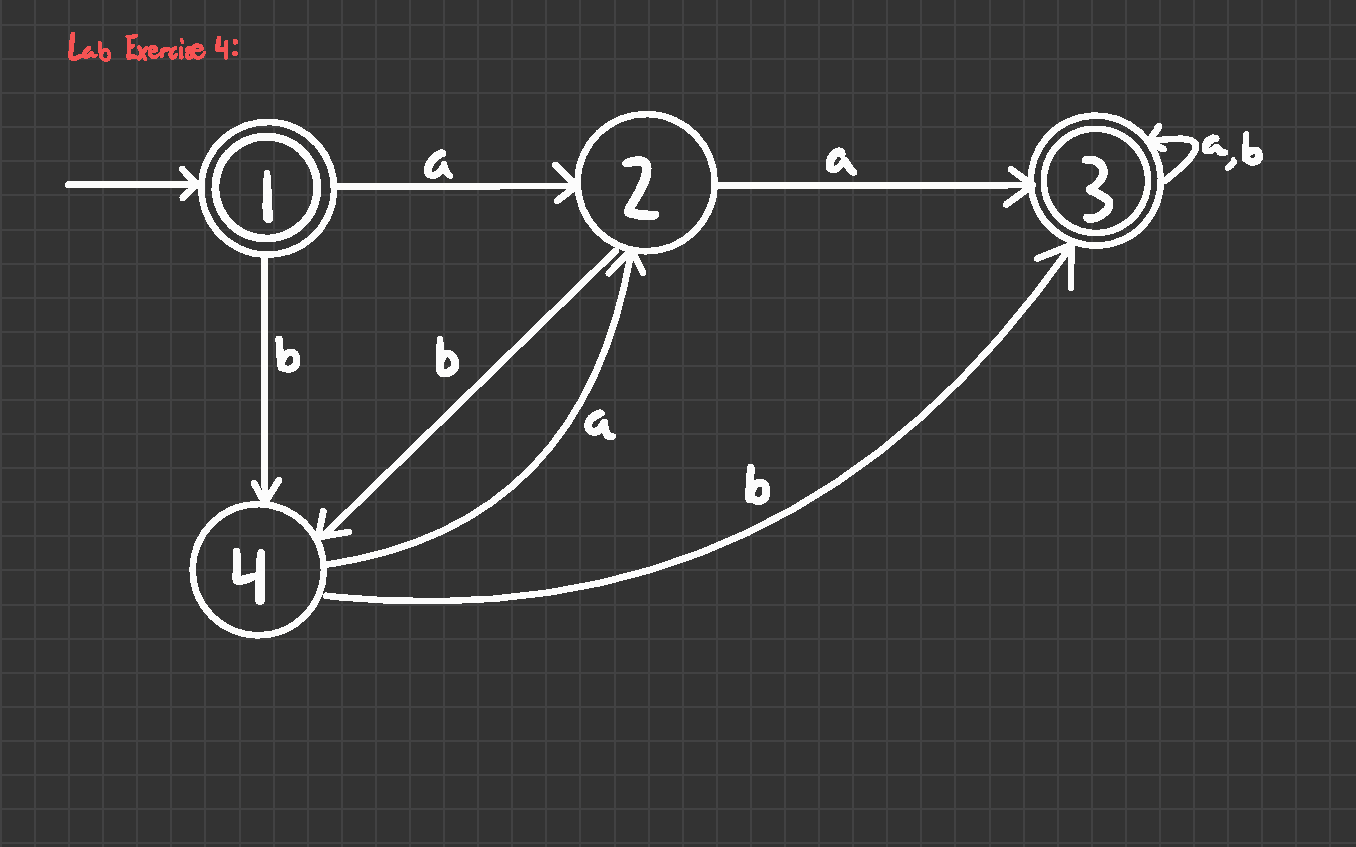
\includepdf[pages=-]{attachments/CPSC406_HW2.pdf}

\subsubsection*{Comments and Questions}

I occasionally find myself struggling to recognize the pattern when first looking at a new DFA. Is there an insightful method or trick to recognizing these patterns more easily?

\subsection{Week 4}

\subsubsection*{Notes}

\subsubsection*{Homework 3}

\underline{Homework 1}

1. The language of the automata A2 can be described as starting with an a and having an odd length. Any b's that may occur must do so from state 2. This can be described as a regular expression $a((a|b)a)*$.

2. The extended transition functions can be evaluated as follows:

A1:
\begin{itemize}
  \item $\delta_1(1, a) = 2$
  \item $\delta_1(2, b) = 4$
  \item $\delta_1(4, a) = 2$
  \item $\delta_1(2, a) = 3$
\end{itemize}

A2:
\begin{itemize}
  \item $\delta_2(1, a) = 2$
  \item $\delta_2(2, b) = 1$
  \item $\delta_2(1, b) = 3$
  \item $\delta_2(3, a) = 3$
\end{itemize}

\underline{Homework 2}

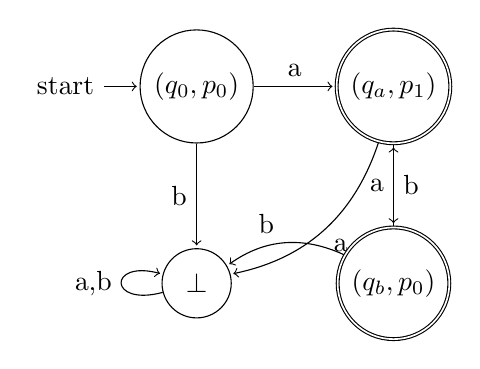
\begin{tikzpicture}[shorten >=1pt,node distance=2.5cm,on grid,auto]
  % Nodes
  \node[state,initial] (q0) {$(q_0,p_0)$};
  \node[state,accepting] (qa) [right=of q0] {$(q_a,p_1)$};
  \node[state,accepting] (qb) [below=of qa] {$(q_b,p_0)$};
  \node[state] (trap) [below=of q0] {$\bot$};
  % Transitions from (q0,p0)
  \path[->]
      (q0) edge node {a} (qa)
           edge node [swap] {b} (trap)
  % Transitions from (q_a,p_1)
      (qa) edge node {b} (qb)
           edge[bend left] node {a} (trap)
  % Transitions from (q_b,p_0)
      (qb) edge node {a} (qa)
           edge[bend right] node [swap] {b} (trap)
  % Trap self-loop
      (trap) edge [loop left] node {a,b} (trap);
\end{tikzpicture}

2. When constructing the product automaton, a word w is processed by both components simultaneously. The word is said to be accepted iff the computation ends in a state $(q,p)$ where q is in F(1) and p is in F(2). This means that w is accepted by both A(1) and A(2), so L(A) can be the intersection between the two. 

3. In the product automaton constrction, the set of states is always $Q_1 * Q_2$ and the transitions are the same. To find an automaton which is the union of the two languages, we change the accepting states. So, a word w is accepted by A' iff it is accepted by at least one of the original automata, which gives L(A') to be the union of L(A1) and L(A2). 

To summarize:

\[
\begin{aligned}
Q &= Q^{(1)}\times Q^{(2)}, \\
\delta((q,p),x) &= (\delta^{(1)}(q,x),\,\delta^{(2)}(p,x)), \\
q_0 &= (q_0^{(1)},q_0^{(2)}), \\
F' &= \Bigl\{(q,p) \in Q^{(1)}\times Q^{(2)} : q\in F^{(1)} \text{ or } p\in F^{(2)}\Bigr\}.
\end{aligned}
\]

\underline{Exercise 2.2.7 - ITALC}

\textbf{Theorem.} Let \(A = (Q,\Sigma,\delta,q_0,F)\) be a DFA and let \(q \in Q\) be such that 
\[
\delta(q,a) = q \quad \text{for all } a \in \Sigma.
\]
Then for all \(w \in \Sigma^*\), \(\hat{\delta}(q,w) = q\).

\textbf{Proof.} We prove by induction on the length of \(w\).

\textit{Base Case:} \(w = \varepsilon\) (the empty string).  
By definition of the extended transition function,
\[
\hat{\delta}(q,\varepsilon) = q.
\]

\textit{Inductive Step:} Assume that for some \(w \in \Sigma^*\), \(\hat{\delta}(q,w) = q\).  
Let \(a \in \Sigma\). Then,
\[
\hat{\delta}(q, wa) = \delta(\hat{\delta}(q, w), a) = \delta(q, a) = q.
\]
Thus, by the principle of induction, for all \(w \in \Sigma^*\), \(\hat{\delta}(q,w) = q\).


\subsubsection*{Comments and Questions}

Do automata with some form of union or intersection have real world applications relating to natural language processing? Could they be used to improve parsing in conversational AI? 

\subsection{Week 5}

\subsubsection*{Notes}
Chapter 3.1-3.2 of ITALC explores regular expressions as a powerful way to more accurately describe formal languages, specifically being useful in various text processing. Regular expressions are built using basic operations such as union, concatenation,and Kleene closure, which combines simple patterns in order to create more complex expressions. These operations and the way they are used is defined through standard set operations. Union is able to combine languages by joining their elements, concatenation makes new strings by combining parts from each language, and Kleene closure allows for the generation of all potential strings. Also, Kleene's algorithm is shown as a structured method in order to change DFAs into regular expressions, usually relying on induction that builds expressions incrementally that represent state transitions. With larger automata, this algorithm can become very computationally expensive. Finally, the transition between regular expressions and automata is bidirectional, meaning you can go from one to the other and back again. 

\subsubsection*{Homework 4}

Homework 1:

Let $\mathcal{A} = (Q, \Sigma, \delta: Q \times \Sigma \to Q, q_0, F)$ be a DFA.

\begin{enumerate}
    \item \textbf{Viewing $\mathcal{A}$ as an NFA:}

    A DFA is a specific case of an NFA where the transition function returns only one next state for each input symbol and state. To show the DFA as an NFA, we make a new transition function $\delta': Q \times \Sigma \to \mathcal{P}(Q)$ sucsoh that:
    \[
    \delta'(q, a) = \{ \delta(q, a) \}
    \]
    This shows that each deterministic transition becomes a singleton set in the NFA transition function. All other components of the DFA remain unchanged:
    \begin{itemize}
        \item $Q' = Q$
        \item $\Sigma$ remains the same
        \item $q_0' = q_0$
        \item $F' = F$
    \end{itemize}

    \item \textbf{General Construction:}

    Given a DFA $\mathcal{A} = (Q, \Sigma, \delta, q_0, F)$, we define an equivalent NFA $\mathcal{A}' = (Q', \Sigma, \delta', q_0', F')$ as follows:
    \begin{align*}
        Q' &= Q \\
        \Sigma' &= \Sigma \\
        q_0' &= q_0 \\
        F' &= F \\
        \delta'(q, a) &= \{ \delta(q, a) \} \quad \text{for all } q \in Q, a \in \Sigma
    \end{align*}

    \item \textbf{Justification:}

    This design ensures that $\mathcal{A}'$ accepts the same language as $\mathcal{A}$. Because each transition in the NFA $\delta'$ corresponds to the DFA's transition , the NFA has exactly one computational path for any given input string, mirroring the DFA. So,
    \[
    L(\mathcal{A}) = L(\mathcal{A}')
    \]
\end{enumerate}

Homework 2: 

\begin{enumerate}
    \item \textbf{Language accepted by $\mathcal{A}$:}  
    The NFA accepts all binary strings that have the substring \texttt{010}.

    \item \textbf{Specification of $\mathcal{A}$:}  
    \begin{itemize}
        \item $Q = \{q_0, q_1, q_2, q_3\}$
        \item $\Sigma = \{0, 1\}$
        \item $q_0$ is the start state
        \item $F = \{q_3\}$
        \item Transition function $\delta$:
        \begin{align*}
            \delta(q_0, 0) &= \{q_0\} \\
            \delta(q_0, 1) &= \{q_0, q_1\} \\
            \delta(q_1, 0) &= \{q_2\} \\
            \delta(q_2, 0) &= \{q_3\}, \quad \delta(q_2, 1) = \{q_1\} \\
            \delta(q_3, 0) &= \{q_3\}, \quad \delta(q_3, 1) = \{q_3\}
        \end{align*}
    \end{itemize}

    \item \textbf{Extended transition: compute $\hat{\delta}(q_0, 10110)$ step-by-step:}
    \begin{itemize}
        \item Step 0: $\{q_0\}$
        \item Read 1: $\{q_0, q_1\}$
        \item Read 0: $\{q_0, q_2\}$
        \item Read 1: $\{q_0, q_1\}$
        \item Read 1: $\{q_0, q_1\}$
        \item Read 0: $\{q_0, q_2\}$
        \item Final result: $\hat{\delta}(q_0, 10110) = \{q_0, q_2\}$
    \end{itemize}

    \item \textbf{All paths for $v = 1100$ and $w = 1010$:}

    \textbf{Step-by-step for $v = 1100$:}
    \begin{itemize}
        \item Start at $\{q_0\}$
        \item Read 1: $\{q_0, q_1\}$
        \item Read 1: $\{q_0, q_1\}$
        \item Read 0: $\{q_0, q_2\}$
        \item Read 0: $\{q_0, q_3\}$ → accepted
    \end{itemize}

    \textbf{Step-by-step for $w = 1010$:}
    \begin{itemize}
        \item Start at $\{q_0\}$
        \item Read 1: $\{q_0, q_1\}$
        \item Read 0: $\{q_0, q_2\}$
        \item Read 1: $\{q_0, q_1\}$
        \item Read 0: $\{q_0, q_2\}$ → rejected
    \end{itemize}

    \textbf{Common diagram of all paths:}

    \begin{center}
    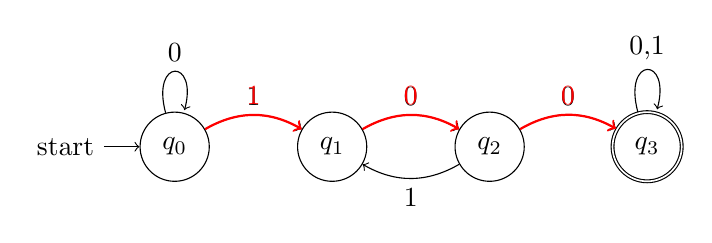
\begin{tikzpicture}[->, node distance=2cm, on grid, auto]
      \node[state, initial] (q0) {$q_0$};
      \node[state] (q1) [right=of q0] {$q_1$};
      \node[state] (q2) [right=of q1] {$q_2$};
      \node[state, accepting] (q3) [right=of q2] {$q_3$};

      \path (q0) edge [loop above] node {0} (q0)
            (q0) edge [bend left] node {1} (q1)
            (q1) edge [bend left] node {0} (q2)
            (q2) edge [bend left] node {1} (q1)
            (q2) edge [bend left] node {0} (q3)
            (q3) edge [loop above] node {0,1} (q3);

      % Highlight sample path for v = 1100
      \draw[red, thick, ->] (q0) to[bend left=30] node {1} (q1);
      \draw[red, thick, ->] (q1) to[bend left=30] node {0} (q2);
      \draw[red, thick, ->] (q2) to[bend left=30] node {0} (q3);
    \end{tikzpicture}
    \end{center}

    \item \textbf{Powerset construction for DFA $\mathcal{A}^D$:}

    Start from state $\{q_0\}$:
    \begin{itemize}
        \item $\delta(\{q_0\}, 0) = \{q_0\}$
        \item $\delta(\{q_0\}, 1) = \{q_0, q_1\}$
    \end{itemize}
    Continue expanding:
    \begin{itemize}
        \item $\delta(\{q_0, q_1\}, 0) = \{q_0, q_2\}$
        \item $\delta(\{q_0, q_1\}, 1) = \{q_0, q_1\}$
        \item $\delta(\{q_0, q_2\}, 0) = \{q_0, q_3\}$
        \item $\delta(\{q_0, q_2\}, 1) = \{q_0, q_1\}$
        \item $\delta(\{q_0, q_3\}, 0) = \{q_0, q_3\}$, etc.
    \end{itemize}
    Accepting states: all subsets that contain $q_3$

    \item \textbf{Verification and minimization:}  
    $L(\mathcal{A}) = L(\mathcal{A}^D)$ by construction. A simple DFA for the language contains substring '010' has 4 states, so $\mathcal{A}^D$ can be simplified further.
\end{enumerate}

\subsubsection*{Comments and Questions}

How does the powerset construction in Homework 2 show the relationship between DFAs and NFAs, and how does this relate to the transformation approach in Homework 1?

\subsection{Week 6}

\subsubsection*{Notes}

\subsubsection*{Comments and Questions}

\subsection{Week 7}

\subsubsection*{Notes}

\subsubsection*{Homework}

\textbf{DFA Regular Expressions and State Elimination (Exercise 3.2.1)}

Given a transition table:
\begin{center}
\begin{tabular}{|c|c|c|}
\hline
       & 0   & 1   \\ \hline
$\rightarrow q_1$ & $q_2$ & $q_1$ \\ \hline
$q_2$ & $q_3$ & $q_1$ \\ \hline
$*q_3$ & $q_3$ & $q_2$ \\ \hline
\end{tabular}
\end{center}

\medskip

\textbf{a. \(R_{ij}^{(0)}\) (Initial regular expressions with no intermediate states)}\\[1mm]
Let 
\[
R_{ij}^{(0)} = \begin{cases}
\text{the symbol(s) labeling direct transitions from state } i \text{ to state } j,\\[1mm]
\varnothing, \quad \text{if no direct transition,}\\[1mm]
\epsilon, \quad \text{if } i = j.
\end{cases}
\]
Thus,
\[
\begin{array}{rcl}
R_{11}^{(0)} &=& \epsilon, \quad R_{12}^{(0)} = 0, \quad R_{13}^{(0)} = \varnothing,\\[1mm]
R_{21}^{(0)} &=& 1, \quad R_{22}^{(0)} = \epsilon, \quad R_{23}^{(0)} = 0,\\[1mm]
R_{31}^{(0)} &=& \varnothing, \quad R_{32}^{(0)} = 1, \quad R_{33}^{(0)} = 0 \mid \epsilon.
\end{array}
\]

\medskip

\textbf{b. \(R_{ij}^{(1)}\) (Using state \(q_1\) as intermediate)}\\[1mm]
Using the formula
\[
R_{ij}^{(k)} = R_{ij}^{(k-1)} \cup R_{i k}^{(k-1)}\,(R_{kk}^{(k-1)})^*\, R_{kj}^{(k-1)},
\]
with \(q_1\) as the singular intermediate state we get:
\[
\begin{array}{rcl}
R_{11}^{(1)} &=& \epsilon \cup (\epsilon)(\epsilon)^*\epsilon = \epsilon,\\[1mm]
R_{12}^{(1)} &=& 0 \cup (\epsilon)(\epsilon)0 = 0,\\[1mm]
R_{13}^{(1)} &=& \varnothing \cup (\epsilon)(\epsilon)\varnothing = \varnothing,\\[1mm]
R_{21}^{(1)} &=& 1 \cup (1)(\epsilon)^*\epsilon = 1,\\[1mm]
R_{22}^{(1)} &=& \epsilon \cup (1)(\epsilon)0 = 10,\\[1mm]
R_{23}^{(1)} &=& 0 \cup (1)(\epsilon)\varnothing = 0,\\[1mm]
R_{31}^{(1)} &=& \varnothing \cup (1)(\epsilon)^*\epsilon = \varnothing,\\[1mm]
R_{32}^{(1)} &=& 1 \cup (1)(\epsilon)0 = 1,\\[1mm]
R_{33}^{(1)} &=& 0 \cup (1)(\epsilon)\varnothing = 0.
\end{array}
\]

\medskip

\textbf{c. \(R_{ij}^{(2)}\) (Using \(q_1\) and \(q_2\) as intermediates)}\\[1mm]
Now we add \(q_2\) as an intermediate state:
\[
\begin{array}{rcl}
R_{11}^{(2)} &=& \epsilon \cup 0\,(10)^*\,1,\\[1mm]
R_{12}^{(2)} &=& 0 \cup 0\,(10)^*\,10,\\[1mm]
R_{13}^{(2)} &=& 0\,(10)^*\,0,\\[1mm]
R_{21}^{(2)} &=& 1 \cup 10\,(10)^*\,1,\\[1mm]
R_{22}^{(2)} &=& 10\,(10)^*\,10 \cup \epsilon,\\[1mm]
R_{23}^{(2)} &=& 0 \cup 10\,(10)^*\,0,\\[1mm]
R_{31}^{(2)} &=& \varnothing \cup 1\,(10)^*\,1,\\[1mm]
R_{32}^{(2)} &=& 1 \cup 1\,(10)^*\,10,\\[1mm]
R_{33}^{(2)} &=& 0 \cup 1\,(10)^*\,0.
\end{array}
\]

\medskip

\textbf{d. Regular Expression for the Language}\\[1mm]
Start state: \(q_1\) \quad Final state: \(q_3\).\\[1mm]
The regex is \(R_{13}^{(2)}\), so
\[
R = 0\,(10)^*\,0.
\]

\medskip

\textbf{e. Transition Diagram and State Elimination (eliminate \(q_2\))}\\[1mm]
A simpler diagram of the DFA is:
\[
q_1 \xrightarrow{0} q_2 \xrightarrow{0} q_3\quad (\text{final})
\]
with loops and additional transitions that are indicated in the original DFA. After getting rid of \(q_2\), the path from \(q_1\) to \(q_3\) becomes:
\[
(1 \cup 01)00(0),
\]
so final regular expression becomes
\[
R = (1 \cup 01)00(0).
\]

\bigskip

\textbf{DFA Regular Expressions and State Elimination (Exercise 3.2.2)}

Given the transition table:
\begin{center}
\begin{tabular}{|c|c|c|}
\hline
       & 0   & 1   \\ \hline
$\rightarrow q_1$ & $q_2$ & $q_3$ \\ \hline
$q_2$ & $q_1$ & $q_3$ \\ \hline
$*q_3$ & $q_2$ & $q_1$ \\ \hline
\end{tabular}
\end{center}

\medskip

\textbf{a. \(R_{ij}^{(0)}\) (Initial regular expressions with no intermediate states)}\\[1mm]
Let
\[
\begin{array}{rcl}
R_{11}^{(0)} &=& \epsilon, \quad R_{12}^{(0)} = 0, \quad R_{13}^{(0)} = 1,\\[1mm]
R_{21}^{(0)} &=& 0, \quad R_{22}^{(0)} = \epsilon, \quad R_{23}^{(0)} = 1,\\[1mm]
R_{31}^{(0)} &=& 1, \quad R_{32}^{(0)} = 0, \quad R_{33}^{(0)} = \epsilon.
\end{array}
\]

\medskip

\textbf{b. \(R_{ij}^{(1)}\) (Using \(q_1\) as intermediate)}\\[1mm]
Apply:
\[
R_{ij}^{(1)} = R_{ij}^{(0)} \cup R_{i1}^{(0)}\,(R_{11}^{(0)})^*\,R_{1j}^{(0)}.
\]
This gives:
\[
\begin{array}{rcl}
R_{11}^{(1)} &=& \epsilon \cup \epsilon\cdot\epsilon\cdot\epsilon = \epsilon,\\[1mm]
R_{12}^{(1)} &=& 0 \cup \epsilon\cdot\epsilon\cdot 0 = 0,\\[1mm]
R_{13}^{(1)} &=& 1 \cup \epsilon\cdot\epsilon\cdot 1 = 1,\\[1mm]
R_{21}^{(1)} &=& 0 \cup 0\cdot\epsilon\cdot\epsilon = 0,\\[1mm]
R_{22}^{(1)} &=& \epsilon \cup 0\cdot\epsilon\cdot 0 = \epsilon \cup 00,\\[1mm]
R_{23}^{(1)} &=& 1 \cup 0\cdot\epsilon\cdot 1 = 1 \cup 01,\\[1mm]
R_{31}^{(1)} &=& 1 \cup 1\cdot\epsilon\cdot\epsilon = 1,\\[1mm]
R_{32}^{(1)} &=& 0 \cup 1\cdot\epsilon\cdot 0 = 0 \cup 10,\\[1mm]
R_{33}^{(1)} &=& \epsilon \cup 1\cdot\epsilon\cdot 1 = \epsilon \cup 11.
\end{array}
\]

\medskip

\textbf{c. \(R_{ij}^{(2)}\) (Using \(q_1\) and \(q_2\) as intermediates)}\\[1mm]
Apply:
\[
R_{ij}^{(2)} = R_{ij}^{(1)} \cup R_{i2}^{(1)}\,(R_{22}^{(1)})^*\,R_{2j}^{(1)}.
\]
For example:
\[
\begin{array}{rcl}
R_{11}^{(2)} &=& \epsilon \cup 0\,( (\epsilon \cup 00) )^*\;0,\\[1mm]
R_{12}^{(2)} &=& 0 \cup 0\,( (\epsilon \cup 00) )^*\;(\epsilon \cup 00),\\[1mm]
R_{13}^{(2)} &=& 1 \cup 0\,( (\epsilon \cup 00) )^*\;(1 \cup 01),
\end{array}
\]
and in a similar manner for the other entries.

\medskip

\textbf{d. Regular Expression for the Language}\\[1mm]
Start state: \(q_1\) \quad Final state: \(q_3\).\\[1mm]
Thus,
\[
R = R_{13}^{(2)} = 1 \cup 0\,( (\epsilon \cup 00) )^*(1 \cup 01).
\]

\medskip

\textbf{e. Transition Diagram and State Elimination (eliminate \(q_2\))}\\[1mm]
A simplified diagram is as follows:
\[
q_1 \xrightarrow{0} q_2 \xrightarrow{0} q_1 \quad \text{and} \quad q_3 \xleftarrow{1} q_3.
\]
By getting rid of \(q_2\) and considering the other paths:
\[
q_1 \xrightarrow{0} q_2 \xrightarrow{1} q_3 \quad \Rightarrow \quad 01,
\]
\[
q_1 \xrightarrow{0} q_2 \xrightarrow{0} q_1 \quad \Rightarrow \quad 00 \text{ (loop)},
\]
the final regex becomes:
\[
R = \left( 1 \cup 0(00)^*1 \right).
\]

\bigskip

\textbf{DFA Minimization (Exercise 4.4.1)}

Given the transition table:
\begin{center}
\begin{tabular}{|c|c|c|}
\hline
       & 0   & 1   \\ \hline
$\rightarrow A$ & $B$ & $A$ \\ \hline
$B$ & $A$ & $C$ \\ \hline
$C$ & $D$ & $B$ \\ \hline
$*D$ & $D$ & $A$ \\ \hline
$E$ & $D$ & $F$ \\ \hline
$F$ & $G$ & $E$ \\ \hline
$G$ & $F$ & $G$ \\ \hline
$H$ & $G$ & $D$ \\ \hline
\end{tabular}
\end{center}

\medskip

\textbf{a. Table of Distinguishabilities}\\[1mm]
We make a lower-triangular table marking different pairs of states.\\[1mm]
\textbf{Step 1:} Mark all the pairs that have one state as final (\(D\)) and the other as non-final.\\[1mm]
\textbf{Step 2:} Propagate markings by checking transitions.\\[1mm]
Final table (checkmark = marked/inequivalent, blank = equivalent):
\[
\begin{array}{c|cccccccc}
& A & B & C & D & E & F & G & H\\ \hline
B & \checkmark &  &  &  &  &  &  &  \\
C & \checkmark & \checkmark &  &  &  &  &  &  \\
D & \checkmark & \checkmark & \checkmark &  & \checkmark & \checkmark & \checkmark & \checkmark \\
E & \checkmark & \checkmark & \checkmark & \checkmark &  &  &  &  \\
F & \checkmark & \checkmark & \checkmark & \checkmark & \checkmark &  &  &  \\
G & \checkmark & \checkmark & \checkmark & \checkmark & \checkmark & \checkmark &  &  \\
H & \checkmark & \checkmark & \checkmark & \checkmark & \checkmark & \checkmark & \checkmark &  \\
\end{array}
\]
The unmarked (equivalent) states are \(E\), \(F\), and \(G\).

\medskip

\textbf{b. Minimum-State Equivalent DFA}\\[1mm]
Merge equal states:
\[
[E, F, G] \to \texttt{EFG}.
\]
The new transition table is:
\begin{center}
\begin{tabular}{|c|c|c|c|}
\hline
State & 0   & 1   & Accept? \\ \hline
\(A\) & \(B\) & \(A\) & No \\ \hline
\(B\) & \(A\) & \(C\) & No \\ \hline
\(C\) & \(D\) & \(B\) & No \\ \hline
\(D\) & \(D\) & \(A\) & Yes \\ \hline
\(\texttt{EFG}\) & \(\texttt{EFG}\) & \(\texttt{EFG}\) & No \\ \hline
\(H\) & \(\texttt{EFG}\) & \(D\) & No \\ \hline
\end{tabular}
\end{center}

\bigskip

\textbf{DFA Minimization (Exercise 4.4.2)}

Given the transition table:
\begin{center}
\begin{tabular}{|c|c|c|}
\hline
       & 0   & 1   \\ \hline
$\rightarrow A$ & \(B\) & \(E\) \\ \hline
\(B\) & \(C\) & \(F\) \\ \hline
\(*C\) & \(D\) & \(H\) \\ \hline
\(D\) & \(E\) & \(I\) \\ \hline
\(E\) & \(F\) & \(H\) \\ \hline
\(*F\) & \(G\) & \(B\) \\ \hline
\(G\) & \(H\) & \(B\) \\ \hline
\(H\) & \(I\) & \(C\) \\ \hline
\(*I\) & \(A\) & \(E\) \\ \hline
\end{tabular}
\end{center}

\medskip

\textbf{a. Table of Distinguishabilities}\\[1mm]
Final states: \(C\), \(F\), and \(I\).\\[1mm]
Mark all the pairs with one final and one non-final state, then make distinctions. The final table (checkmark = distinguishable) is:
\[
\begin{array}{c|ccccccccc}
 & A & B & C & D & E & F & G & H & I \\ \hline
B & \checkmark &  &  &  &  &  &  &  &  \\
C & \checkmark & \checkmark &  &  &  &  &  &  &  \\
D & \checkmark & \checkmark & \checkmark &  &  &  &  &  &  \\
E & \checkmark & \checkmark & \checkmark & \checkmark &  &  &  &  &  \\
F & \checkmark & \checkmark & \checkmark & \checkmark & \checkmark &  &  &  &  \\
G & \checkmark & \checkmark & \checkmark & \checkmark & \checkmark & \checkmark &  &  &  \\
H & \checkmark & \checkmark & \checkmark & \checkmark & \checkmark & \checkmark & \checkmark &  &  \\
I & \checkmark & \checkmark & \checkmark & \checkmark & \checkmark & \checkmark & \checkmark & \checkmark &  \\
\end{array}
\]
The equivalent states (unmarked) are \(C\), \(F\), and \(I\), which we merge as:
\[
[C, F, I] \to \texttt{CFI}.
\]

\medskip

\textbf{b. Minimum-State Equivalent DFA}\\[1mm]
The new transition table becomes:
\begin{center}
\begin{tabular}{|c|c|c|c|}
\hline
State & 0   & 1   & Accept? \\ \hline
\(A\) & \(B\) & \(E\) & No \\ \hline
\(B\) & \(\texttt{CFI}\) & \(\texttt{CFI}\) & No \\ \hline
\(\texttt{CFI}\) & \(D\) & \(H\) & Yes \\ \hline
\(D\) & \(E\) & \(\texttt{CFI}\) & No \\ \hline
\(E\) & \(\texttt{CFI}\) & \(H\) & No \\ \hline
\(G\) & \(H\) & \(B\) & No \\ \hline
\(H\) & \(\texttt{CFI}\) & \(\texttt{CFI}\) & No \\ \hline
\end{tabular}
\end{center}
This minimized DFA reduces the original 9 states to 7 states with the final state being \(\texttt{CFI}\).

\subsubsection*{Comments and Questions}

In Exercise 3.2.1, how does the order of state elimination change the final regular expression’s structure, and could a different order get us to a more simplified form?

\section{Synthesis}

\section{Evidence of Participation}

\section{Conclusion}\label{conclusion}

\begin{thebibliography}{99}
\bibitem[BLA]{bla} Author, \href{https://en.wikipedia.org/wiki/LaTeX}{Title}, Publisher, Year.
\end{thebibliography}

\end{document}